The most common type of radiation therapy is external beam therapy, which is characterised
by directing ionizing radiation from the outside into the patient's body. Treatment planning is an
integral part of radiation therapy treatment, performed before the actual patient treatment using specialized software. The treatment planning process aims to simulate the dose deposition within the patient's body and to optimize the dose distribution according to clinical objectives and constraints that define a trade-off between tumour irradiation and normal tissue sparing. 
\subsection{Treatment Planning Process}
The treatment planning process involves several steps, which are outlined below in Figure~\ref{fig:tpworkflow}.

\begin{figure}[H]
    \centering
    \scalebox{0.78}{%
    \begin{tikzpicture}[
        node distance = 5mm and 8mm,
        box/.style = {rectangle, rounded corners=4pt,
                      draw=white, fill=black!80,
                      text=white, font=\small\bfseries,
                      text width=23mm, minimum height=12mm,
                      align=center},
        arr/.style = {->, >=stealth, thick, orange!90!red},
    ]
        %% Row 1 (left to right)
        \node[box] (pos)  {Patient positioning and immobilization};
        \node[box, right=of pos]  (img)  {Image acquisition and registration};
        \node[box, right=of img]  (geo)  {Treatment geometry definition};
        \node[box, right=of geo]  (init) {Initialize plan modality and geometry};

        %% Row 2 (right to left)
        \node[box, below=of pos]  (del)  {Plan delivery};
        \node[box, right=of del]  (qa)   {Quality assurance};
        \node[box, right=of qa]   (prep) {Prepare plan for delivery};
        \node[box, right=of prep] (dose) {Dose calculation and evaluation};
        \node[box, right=of dose] (opt)  {Treatment plan optimization};

        %% Dotted blue bounding box around TPS-internal steps (excludes image acquisition)
        \node[draw=blue!70, dashed, thick, rounded corners=6pt,
              inner sep=4mm,
              fit=(geo)(init)(prep)(dose)(opt),
              label={[blue!70, font=\footnotesize, yshift=1mm]}] {};

        %% Arrows — row 1
        \draw[arr] (pos)  -- (img);
        \draw[arr] (img)  -- (geo);
        \draw[arr] (geo)  -- (init);

        %% init down to opt
        \draw[arr] (init) -- (opt);

        %% Arrows — row 2 (right to left)
        \draw[arr] (opt)  -- (dose);
        \draw[arr] (dose) -- (prep);
        \draw[arr] (prep) -- (qa);
        \draw[arr] (qa)   -- (del);

        %% Feedback arrow: dose back to opt (orange loop below)
        \draw[arr, orange!90!red]
            (dose.south) -- ++(0,-6mm) -| (opt.south);
    \end{tikzpicture}}
    \caption{The treatment planning workflow. The dotted blue region represents the TPS-internal steps covered in this experiment.}
    \label{fig:tpworkflow}
\end{figure}

\subsubsection{Treatment Plan Prescribing and reporting}

In external photon beam radiotherapy, prescription and reporting require clear definition of target-related volumes and dose-reporting quantities so that treatment intent is unambiguous and reproducible \cite{gibbons_khans_2020}.

\begin{figure}[H]
    \centering
    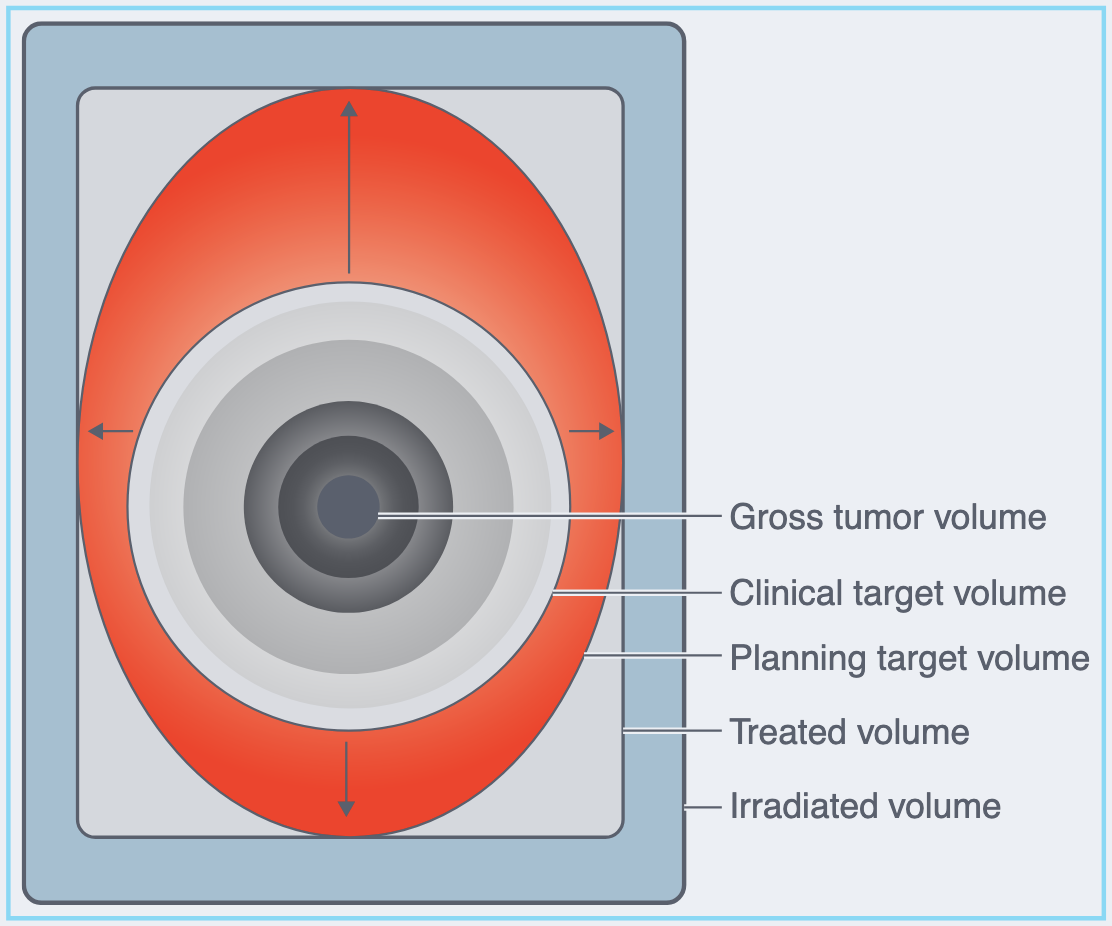
\includegraphics[width=0.5\textwidth]{Figures/TheoryFIgures/Tumour.png}
    \caption{ICRU target and dose specification concepts used in treatment plan prescribing and reporting.}
    \label{fig:tumour_volume_specification}
\end{figure}

\begin{itemize}
    \item \textbf{Gross Tumor Volume (GTV):} The gross demonstrable extent of malignant disease identified clinically or through imaging.
    \item \textbf{Clinical Target Volume (CTV):} GTV plus regions suspected to contain microscopic disease; it represents the true tissue volume that must receive adequate dose.
    \item \textbf{Internal Target Volume (ITV):} The volume obtained by adding an internal margin to CTV to account for internal physiological motion and shape/position variation.
    \item \textbf{Planning Target Volume (PTV):} CTV (or ITV) plus setup margin to account for patient positioning and machine-related geometric uncertainties during treatment delivery.
    \item \textbf{Organ at Risk Volume (PRV / OAR volume):} A margin-expanded planning representation of an organ at risk, used to better protect normal tissues under motion and setup uncertainty.
    \item \textbf{Irradiated Volume:} The tissue volume receiving a clinically significant dose level (commonly a threshold relative to prescription dose), usually larger than treated volume.
    \item \textbf{Maximum Target Dose:} The highest absorbed dose within the target region that is considered clinically meaningful.
    \item \textbf{Minimum Target Dose:} The lowest absorbed dose found within the target region.
    \item \textbf{Mean Target Dose:} The arithmetic average dose in the target volume, typically calculated over sampled dose points/voxels.
    \item \textbf{Median Target Dose:} The central dose value within the target dose distribution (50th percentile).
    \item \textbf{Modal Target Dose:} The most frequently occurring dose value in the target dose distribution.
    \item \textbf{Hot Spots:} A hot spot is an area outside the target that receives a higher dose than the specified target dose. Like the maximum target dose, a hot spot is considered clinically meaningful only if it covers an area of at least 2 cm$^2$.
\end{itemize}

These definitions provide a standard framework for prescription, comparison, and reporting of treatment plans across institutions \cite{gibbons_khans_2020}.


\subsubsection{Treatment plan and geometry definition}

After prescription, treatment planning begins with defining target volumes and critical organs using CT, MRI, or PET imaging. This 3D delineation process, known as contouring or segmentation, identifies structural borders which can be digitally represented as binary masks or triangular meshes. While manual or semi-automated thresholding techniques have traditionally been used, modern workflows increasingly rely on automated segmentation tools to improve efficiency and consistency. These advanced tools encompass atlas-based segmentation---utilizing deformable image registration from a library of clinical cases---as well as artificial intelligence (AI) methods based on convolutional neural networks (CNNs). Despite these advancements, all automated segmentations necessitate thorough manual review and clinical editing to ensure precision before treatment delivery.


\subsubsection{Creation of a treatment plan}

\subsubsection{Dose display and analysis tools}
1. \textbf{Isodose curves}

2. \textbf{Dose distribution in axial, sagittal, and coronal planes(3D dose distribution)}

3. \textbf{Dose-volume histograms (DVHs)}
\subsubsection{Intensity modulation}
1. \textbf{Forward and Inverse Planning}

2. \textbf{The rationale for intensity modulation}

3. \textbf{Simple optimization mathematics}
\subsection{matRad Workflow}

\texttt{matRad} is an open-source dose calculation and optimization toolkit developed entirely in MATLAB, explicitly designed for three-dimensional intensity-modulated radiation therapy (IMRT) research and educational purposes \cite{wieser_development_2017}. The software features a highly modular and sequential design that mirrors a clinical treatment planning environment. After importing patient anatomical models—either from external DICOM data or utilizing pre-loaded datasets like the CORT database—users can systematically compute and evaluate plans. The standard \texttt{matRad} workflow comprises four primary sequential processes:

\begin{figure}[H]
    \centering
    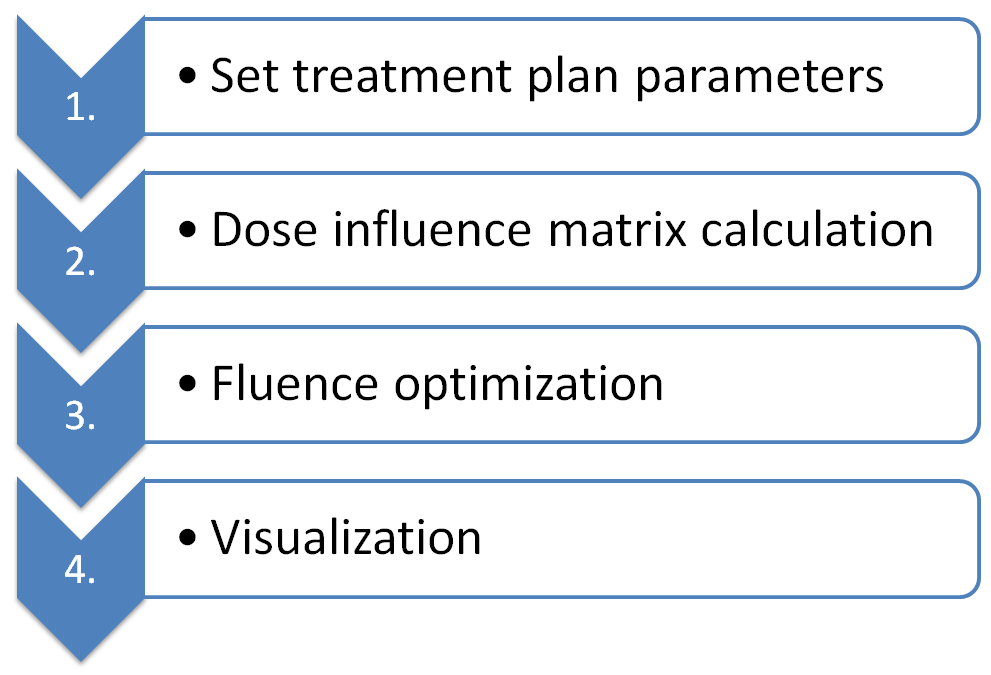
\includegraphics[width=0.7\textwidth]{Figures/TheoryFIgures/matRad_steps.png}
    \caption{The modular workflow of \texttt{matRad} illustrating the sequential progression from plan parameterization to final visualization.}
    \label{fig:matrad_workflow}
\end{figure}

\begin{enumerate}
    \item \textbf{Set Treatment Plan Parameters:} The workflow begins by initializing the dosimetric and geometric constraints. In this module, planners configure the desired irradiation modality (photons, scanned protons, or scanned carbon ions), define beam geometries including gantry and couch angles, establish grid resolutions, and delineate the requisite physical targets alongside proximate Organs at Risk (OARs) using the provided structural data.
    
    \item \textbf{Dose Influence Matrix Calculation:} Once the spatial architecture is parameterized, \texttt{matRad} runs physical dose calculation algorithms to formulate the dose influence matrix (the $D_{ij}$ matrix). This process computes the differential dose contributed by every individual non-zero beamlet or scanning pencil beam to each corresponding voxel within the volumetric CT grid. For scanned carbon ions, this module concomitantly calculates the physical dose and the associated Relative Biological Effectiveness (RBE).
    
    \item \textbf{Fluence Optimization:} Following the matrix derivation, the system engages its central inverse planning engine. The fluence optimization module applies numerical optimization routines to resolve the ideal intensity weights of the multiple independent beamlets. By balancing customized objective functions and physiological penalties—maximizing conformality to the tumour volume while stringently minimizing dose to healthy tissue structures—the optimizer converges upon a clinically acceptable fluence distribution.
    
    \item \textbf{Visualization:} To conclude the workflow, the visualization engine structurally renders the outcome. Treatment planners are provided graphical user interfaces (GUI) to visually interpret the 3D dose distributions overlaid on axial, coronal, and sagittal CT slices. Furthermore, the module displays quantitative plan evaluations, such as Dose-Volume Histograms (DVHs), permitting a thorough and rigorous assessment of the resultant treatment topology \cite{wieser_development_2017}.
\end{enumerate}
